\chapter{Terminology Used}
\section*{Object-Relational Mapping}

Object-relational mapping is a way to access relational data in an
object-centred programming language \cite{agile-mapping-objects}. The primary
purpose is manipulating data without switching concepts from object-oriented
paradigms to the relational representation of data in which most databases
operate. The scope of this translation layer can (as shown later in this work)
vary. Different people define packages as ORMs while providing diverse levels of
functionality \cite{artima-abstractions}.

At its base level, ORM provides an intermediary layer between applications' OOP
model and database which is usually relational (but can be graph or document
focused). The layer allows the developer to work with objects in the code, while
the package translates it into a relational structure when saved to the
database. These packages are often used on projects that are heavily connected
to a database model, as ORMs are most beneficial when using a database is
commonplace. When used only occasionally, it usually brings too expansive a
setup to translate into gains in code readability and maintenance costs compared
to executing premade SQL queries \cite{Torres_Galante_Pimenta_Martins_2017}.

In addition to the basic functionality of translating between different styles
of data representation, ORMs often include functionality such as connection
pooling, support for read-only data replications, caching, or database
migrations. When using such modules, developers can avoid writing boilerplate
code that is typically required.


\section*{SQL Query Builder}

SQL query builder is derived from its function to create SQL queries and OOP
pattern, which it implements, called \enquote{builder}. Object-oriented
programming design patterns are reusable solutions commonly encountered during
software development in OOP languages. These patterns propose interactions
between objects and their internal structure. There is no single authority on
how these patterns are defined, nor a comprehensive list of these patterns, as
every author prioritises different patterns and functionalities
\cite{fowler-patterns-2003}.

The Builder pattern is one such pattern, providing API for the complex creation
process of objects. This pattern is one of the 23 defined in "Design Patterns"
by Erich Gamma, Richard Helm, Ralph Johnson, and John Vlissides
\cite{gamma-design-1995}, which has been highly influential in software
engineering. Its purpose is to separate the creation of an object from its
representation, allowing for the separation of parts that initially were parts
of one construction method into several.

SQL Query is made up of several clauses, which each serve distinct functions.
For example, the \texttt{SELECT} clause specifies which columns are to be
retrieved, and the \texttt{FROM} clause specifies which table or tables the
columns should be \cite{postgres-lexer}. Once the builder pattern is applied to
the SQL query, each of these clauses (or even smaller fragments) can be created
by calling the Builder's methods, creating a programmatic way to create SQL
queries. The Builder also allows developers to abstract minor differences
between different SQL implementations.

As the ability to create queries based on multiple criteria is one of the basic
functionalities of ORMs, they are almost always built on some query builder.
These can be available standalone or fully integrated into the ORM package.
Often, query builders are sufficient for the purposes of database access in most
applications, so they were included in the comparison. While they certainly lack
feature sets and, compared to ORMs, query builders usually require SQL
knowledge, they can be easier to set up and maintain while also being faster and
allowing fine-tuned adjustments to a query.

\section*{PostgreSQL}
One of the most popular database engines today, PostgreSQL, is an open-source
object-relational database management system. Originally developed under the
name Postgres \cite{postres-about} (short for Post-Ingres) as a new generation
after a successful relational database called Ingress, it was first released
under this name in 1989. After several years of development at the University of
California at Berkeley, the name was changed to focus on SQL compliance. The
whole project moved to open-source, community-focused development in 1996.
Currently, the project is maintained by The PostgreSQL Global Development Group,
and releases and source code are provided under an open-source BSD-style licence
free of charge.

PostgreSQL is, at the time of writing, one of the most popular SQL databases
available, owing to its widespread adoption to reliability and high scalability
while supporting most of the SQL standard and being fully ACID compliant
\cite{postgres-transaction}. ACID is an acronym for Atomicity, Consistency,
Isolation, and Durability, which are four fundamental tenets specifying
properties for reliability and consistency of transactions.

Some of the features that often make PostgreSQL stand out amongst other RDBMS
are its support for many different and advanced data types
\cite{postgres-datatypes} out of the box, such as the ability to natively store
JSON objects and arrays, XML data or geometric types. With extensibility being a
significant focus, a lot of functionality can be installed or optionally
enabled, further improving the reach and applicability.

There are extensive implementations of the API for many programming languages,
including C \cite{libpq}, Python \cite{psycopg2}, Java \cite{pgJDBC}, and
JavaScript \cite{node-postgres}. PostgreSQL also offers extensive documentation
of both its API and internal functionality, which supports its growth and
popularity.

\section*{Lazy loading}
Lazy loading is a technique for optimizing data retrieval to increase
application performance \cite{webPerformanceMDN}. It is a strategy consisting of
only loading data when it is needed rather than all at once, therefore reducing
the initial load in exchange for the need to do additional loading later. Lazy
loading is usually achieved by breaking down larger datasets into smaller ones
and loading each one only when necessary. Such practice is commonplace in web
development, as asset sizes (such as images or JavaScript) have only grown in
the evolution of the web.

Some of the most common implementations of Lazy Loading come in the way of only
loading low-quality images unless the user is focused on them or splitting code
into multiple files, which are fetched when necessary, providing quick first
page-load time at the cost of adding additional requests
\cite[p.~200]{fowler-patterns-2003}.

When talking about ORMs and database access, lazy loading usually takes place as
replacing data retrieval from an object with a call to retrieve the data from
the database. In other words, the data of the database object does not need to
be loaded when the object representation or its part is created in the program.
This technique is often used for loading relations so that only one table needs
to be queried to create the essential representation of the object while
skipping the need for additional fetches or joins that are only invoked once
needed.

\section*{Eager loading}
Eager loading is the programming practice of loading all the required data at
once, optimizing the number of requests that must be made to retrieve everything
\cite{sequelize-eager-loading}. This is done with the expectation that one
expensive request will minimize the amount of additional data that would need to
be sent between the two parties. This can lead to faster load times and improved
application performance.

It is usually achieved by sending a singular request and caching the data in
memory, even though it might only be needed later. There are obvious downsides
to this, such as higher memory usage or often loading more data than is
necessary. The concept of eager loading is antithetical to the lazy loading
approach, and that is on purpose. Each approach prefers a different focus, and
thus each is fit for different usage; lazy loading is practical when a first
look or first results matter the most, and eager loading is when the focus is on
one large result, which would be slowed down by too many small requests, which
would need to be made for the total result.

In the context of object-relational mapping frameworks, we are most likely to
encounter eager loading when fetching related entities. This way, when there is
an expectation for data about the currently approached entity, the ORM can
optimize the query so that the data are already loaded in memory when it is
requested later.


\section*{Circular dependence}
A common problem in software development, circular dependency occurs when two or
more parts of code depend on each other, making it impossible to resolve their
dependence onto a dependency graph. Such a graph must conform to limits set out
for tree graphs and, therefore, cannot contain a loop. Due to the way how
modules are loaded in Node.JS \cite{commonjsModulesNode}, such a problem would
lead to a deadlock and is therefore resolved by trying to run the modules in a
specific order. However, such an approach is only sometimes feasible, so other
solutions must be used. The issue of circular dependency is also present in the
compilation because, while TypeScript does allow asynchronous references of
types between files using \texttt{import type} term \cite{typescript-modules},
if we need to import not only the type but also the value, TypeScript will not
be able to resolve the type, and the compilation will fail. There are many
solutions to this problem, the most common being dependency injection or lazy
loading.

In ORMs and database representation in OOP languages, this problem is generally
connected to the bidirectional nature of relations, as its explicit
representation will inevitably create circular dependency
\cite{melton-empirical-2007}. Therefore, for most schema definitions, there
needs to be a functionality built in that allows users to define bidirectional
relations without sacrificing type safety or encountering a deadlock with
importing modules. 


\section*{Database transaction}
Transaction isolation is a concept used in database management to represent a
unit of work. The transaction is typically a series of one or more database
operations that are supposed to be completed on the all-or-nothing principle. In
addition to performing database queries atomically, the transaction also needs
to provide additional functionality, such as coordination of reads and handling
operations in a reliable and recoverable manner. 

As database transactions are the base for the basic functionalities of modern
RDBMS \cite{haerder-principles-1983}, their handling is essential when
considering the ORM framework. Often an operation can only be performed when the
previous one succeeded or has to be made strictly in order without another
operation having access to the data in between \cite{postgres-transaction}. This
can be achieved only through the database transaction, and support for them is
necessary for many use cases.


\section*{Database connection pool}
A database connection pool is a component that collects and manages several
database connections and allocates them to individual requests to the database.
It works by creating either a fixed number of connections at the beginning or
scaling up the number of connections based on usage. In this way, querying the
database does not have to wait for the connection to be established, and the
request can be routed through the database connection pool to the currently
unused connection \cite{gupta-improving-2017}. Additionally, due to having
multiple connections, multithreaded and asynchronous applications can coordinate
connections to the database. Single connection applications can be stalled while
waiting for a single otherwise non-blocking request, while others could be
served by the database. Such connections must be coordinated with transaction
management, as the transaction is inherently connected with the connection that
spawned it. 


\section*{Read replica}
A read replica is a special kind of database instance, a read-only instance of
the database presenting additional query points for the applications accessing
the database without having to resolve consistency between instances. With usual
databases supporting multiple instances, concurrent writes to alternative
machines could produce an inconsistent state in the database. With a read-only
replica, consistency is not threatened; the only negative is the possibility
that the connections will receive a state that is delayed when the replica is
not synced to the latest consistent state of the primary instance
\cite{postgres-availability}.

Creation and usage of read replicas can significantly speed up database
performance as queries are no longer constrained by single hardware, which
usually bottlenecks query speed. Duplicating the data over two instances can
double disk read speeds; if different physical devices are used, slow sequential
scans over data can run independently and finish faster.


\section*{JavaScript}
A high-level dynamically typed programming language developed in the mid-1990s
at Netscape Communications Corporation to add dynamic content to web pages.
Initially called Mocha, it was later renamed multiple times to finally settle on
JavaScript to use the (at the time very high) popularity of Java
\cite{auth0JavascriptHistory}.

Before JavaScript, websites were almost always purely static documents that were
displayed in web browsers (such as Netscape at the time or Google Chrome or
Firefox currently). The logic for any web application had to be handled purely
on the server side. With the introduction of JavaScript, web pages were able to
be more interactive and dynamic. While initially designed to be used when
writing HTML documents and executed by web browsers, it outgrew its client-side
roots and conquered large parts of the server-side development and even mobile
app and desktop application environments. The advantage of JavaScript is that it
can be a completely full-stack language that provides exact parity of logic
between client and server and allows for significant code portability.

Until the last few years, JavaScript had an exclusive reign over interactive web
content, which made it one of the most used programming languages in the world
\cite{stack-overflow-survey}. With multiple deficiencies known and unfixable
without massive problems with incompatibility, multiple additions which build
atop JavaScript and even whole languages which compile into JavaScript were
developed. Some complied languages are, for example, CoffeeScript
\cite{coffeescript-homepage}, Dart \cite{dart-homepage} or TypeScript
\cite{typescript-homepage}. These languages exist to provide additional features
and functionality that are not easily or at all possible in pure JavaScript.


\section*{ECMAScript}
Soon after the introduction of JavaScript, it became apparent that establishing
standards would be a necessary step for compatibility between implementations in
different web browsers. Following this consensus, Ecma (originally an acronym
for European Computer Manufacturers until 1994 \cite{ecma-mission})
International standards association meeting was held, and the first edition of
the document specifying the new standard specification was adopted in June 1997.

The document, coded under the name ECMA-262 \cite{ecma-262}, is a comprehensive
document that has gone over several versions over the years and specifies the
syntax, semantics, and behaviour of the language. There is also an extensive
description of data types, operators, flow control structures, built-in objects,
and API.

ECMAScript is currently used primarily for client-side scripting, with primary
implementations being those used in web browsers, such as SpiderMonkey (Firefox)
\cite{spidermonkey-documentation}, V8 (Google Chrome, Opera) \cite{v8-homepage}
and JavaScriptCore (Safari) \cite{javascript-core}. Increasingly with new
revisions of the standard, even server-side applications and services have
started migrating to ECMAScript from other standards (primarily CommonJS), but
many constructs are not directly compatible or translatable.


\section*{CommonJS}
One of the alternative specifications which reflected missing functionality in
ECMAScript is CommonJS. Created to establish conventions on modularisation for
JavaScript outside the web browser, it has also standardised several APIs and
internal features \cite{commonjs-spec}. 

Started in 2009 by an engineer at Mozilla, the project was initially called
ServerJS, with its flagship feature being the synchronous loading of modules.
This means that once a module is imported, its exported components are
immediately available to be used \cite{commonjs-introduction}. This simplifies
working with modules and was necessary for the expansion of JS code into
server-side development and is used widely today. 

Since its conception, gripes with the ECMAScript specifications were largely
fixed with further iterations, making it also usable in server-side development.
Popular packages, including those exclusively used in server development, have
migrated their codebase to ECMAScript.


\section*{TypeScript}
A statically typed language built on top of the JavaScript foundation,
TypeScript was developed by Microsoft Corporation with the focus on allowing
developers to catch errors at compile time before the problem is encountered
during runtime, which usually requires extensive testing. TypeScript code is
written in enhanced syntax and then compiled into regular JavaScript, with
several standards supported, including CommonJS and ECMAScript
\cite{typescript-modules}.

TypeScript was designed to address several shortcomings that have been present
in the ecosystem for a lost time, especially when creating large-scale
applications. JavaScript applications are very flexible with their dynamic and
loosely typed nature and prototype usage, but with flexibility comes a large
surface area for errors and mistakes. 

Today, TypeScript is widely used for web development and JavaScript server-side
development. Most popular frameworks provide at least partial support for
TypeScript, and some (such as Angular and React) have even switched to it as the
preferred language. TypeScript has support in many JavaScript-integrated
development environments, such as Microsoft's Visual Studio Code
\cite{typescript-vscode} or JetBrains WebStorm \cite{typescript-webstorm}. With
solid typing comes the ability for more substantial and consistent code
completion, guaranteed automated refactoring, and error checking.

Other projects have tried to fix the same issues as TypeScript fixes. For
example, Dart \cite{dart-homepage}, which is developed by Google, works in the
same way, although further from the traditional syntax. It is also compiled into
standard ECMAScript syntax. However, it never gained the same traction, and its
focus was changed from alternative to JavaScript to the primary language for
development in the multi-platform framework Flutter.


\section*{Node.js}
Node.js is an open-source, cross-platform JavaScript based on the V8 engine,
which was originally developed by Google for Google Chrome. It is designed to
allow for server-side usage of JavaScript, with focus on network applications
\cite{node-about}. Released by Ryan Dahl in 2009 \cite{ryan-node}, it has since
become standard for server-side JavaScript development, especially web
applications. The framework has gained popularity thanks to its alternative
execution model, which separates it from traditional server-side languages.
Instead of spawning different threads or workers for connections, it works with
a non-blocking asynchronous I/O model, where many concurrent connections can be
handled with only a small overhead \cite{orsini_2013}.

This is achieved through asynchronous programming, where multiple tasks can be
executed concurrently without blocking the main execution. Node.js supports
asynchronous programming through the concepts of callbacks and promises.
Callbacks are functions passed as arguments that are executed in finished or
failed states, ensuring that logic can be applied sequentially after the
asynchronous operation is finished. Promises provide a more structured and
object-focused way to handle asynchronous operations and have become the
preferred way. A promise is a representation of value which might not be
available yet, containing a status variable and reference for the result once
achieved, allowing for code execution while the operation status is updated in
the background. When the value of the promise is necessary, the promise can be
checked or awaited by using the async/await constructs
\cite{PromiseJavaScriptMDN_2023}.

While Node.js is currently the most dominant, there are other alternatives
available with their own approaches and focuses. The most popular one is Deno,
also developed by Ryan Dahl, intending to address some of the security and
design issues of Node.js. Deno \cite{Deno}, for example, contains extensive
tools and utilities within its standard library or uses better sandboxing
between modules as supported by V8, the engine on which both it and Node.js run.


\section*{npm}
One of the key benefits of the Node.js ecosystem is the large number of
third-party packages that can be incorporated into projects. For example, many
popular web frameworks, such as Koa or Express.js, are built for Node. Database
drivers are also provided in module form, and therefore there needs to be a tool
which allows users to incorporate such modules into their projects efficiently. 

Originally an acronym for Node Package Manager \cite{npm-old-readme}, the
three-letter name has been retroactively stripped of such meaning
\cite{npm-usage}. The first release was published in 2010, and it has since
become the default Node.js package manager. Npm consists of a command line
client, which is also called npm, and an online database of packages called the
npm registry, which is hosted at \url{www.npmjs.com}. 

Although npm is the default package manager, alternatives that were created with
different focuses and compromises exist, for example, yarn \cite{Yarn}.

\section*{JSON}
JavaScript object notation (JSON) is a lightweight data-interchange format that
is widely used in web development. Introduced as an alternative to the complex
XML format that was previously used, it is based on a subset of JavaScript
representation of values. It consists of key-value pairs in objects, arrays, and
primitive types. One of the main benefits is its simplicity and readability for
humans, which makes it useful for places where data could need to be interpreted
by both humans and machines.

JSON has been standardised in the ECMA-404 \cite{ECMA-404} document by Ecma
International. The document specifies syntax and semantics, ensuring its
reliability, consistency, and portability throughout systems and applications.


\section*{Unit of Work}
Unit of Work is a software design pattern used most commonly in ORMs and similar
frameworks to manage persistence and consistency between application and
database state. The pattern is used to group all database operations relating to
a single transaction or process and only execute the final state, ensuring they
can be performed atomically without requiring lengthy and expensive locking of
database rows or tables or risking deadlocks through database transactions
\cite[p.~184]{fowler-patterns-2003}.

The main idea is to track changes across the object in memory, and instead of
committing every change into the database, only the last state change is
executed. This can be applied not only across one object instance but also
across whole swathes of objects. While atomicity is undoubtedly necessary on
many occasions, and unit of work on the ORM side can significantly reduce the
number of requests to the database, it can also lead to inconsistency when
multiple applications access the database and data which are currently loaded in
memory on one machine are modified by a different one.


\section*{Active record}

\begin{figure}[b]
    \caption{Active pattern class diagram, recreated from Patterns of Enterprise Architecture}
    \centering
    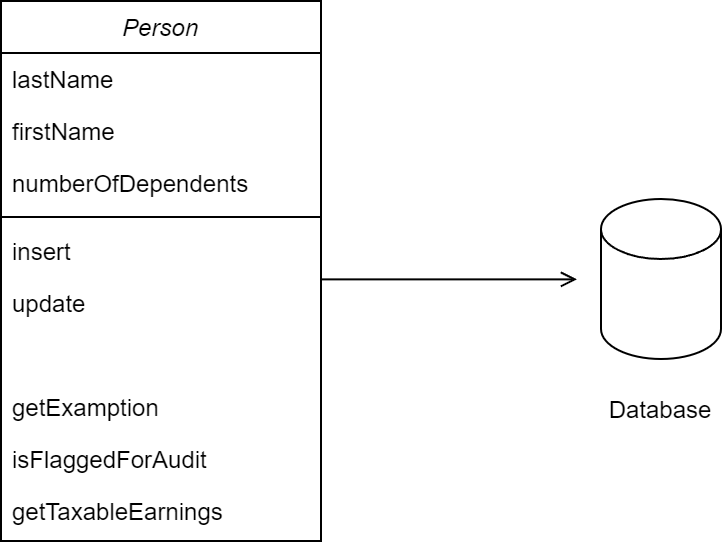
\includegraphics[width=0.6\textwidth]{ActiveRecord}
\end{figure}

The Active Record pattern is a design pattern defined by Martin Fowler in his
book "Patterns of Enterprise Application Architecture" and is commonly used to
represent database records in an application.

The goal of the pattern is to encapsulate logic for interacting with the
database table into a single object. Each instance of the object represents a
single record, and modifications made on it are then usually flushed with a
method call into the database. The base class also provides static methods for
CRUD (create, read, update, delete) operations and possibly additional business
logic \cite[p. 160]{fowler-patterns-2003}.  

The main benefit of the Active Record pattern is a simple and intuitive
interface for objects and tables. Modifications of the object can be made right
on the data in languages, which allow setters and getters on attributes, and
static methods provide a simple gateway to work with the table. 

Limitations of the pattern come in the tight coupling between the application
and database logic, as the object instance is inherently tied to the database
representation. This makes it harder to test the implementation and often
requires additional abstraction or mocking. Additionally, the pattern does not
easily allow for the management of relations, so a database schema with complex
relations might not be able to represent the data easily. 


\section*{Data mapper}

\begin{figure}[b]
    \caption{Data Mapper class diagram, recreated from Patterns of Enterprise Architecture}
    \centering
    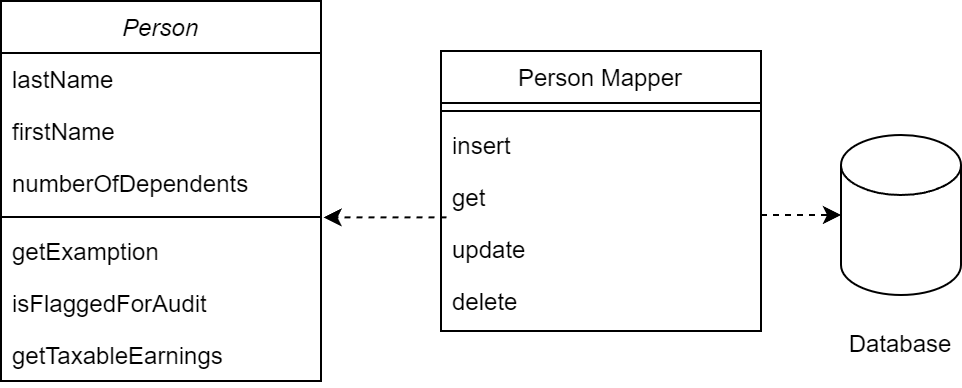
\includegraphics[width=0.8\textwidth]{DataMapper}
\end{figure}

The Data Mapper pattern, as described by Martin Fowler in his seminal work on
enterprise application architectures, provides a clear separation between domain
models and their underlying data storage. This approach enables developers to
create complex and expressive domain models without being constrained by the
relational database schema or various storage options. By decoupling in-memory
representations from the data storage mechanisms, the Data Mapper pattern
promotes a clean separation of concerns and enhanced flexibility in application
design \cite[p. 165]{fowler-patterns-2003}.

Distinguished from the Active Record pattern, the Data Mapper pattern ensures
that business logic and data access responsibilities remain separate. In this
approach, a single entity represents the table or collection, while distinct
entities represent individual records. The Data Mapper serves as a data access
layer that performs operations on the data storage representation without
creating any direct bindings between in-memory objects and the database. This
responsibility is solely managed by the Data Mapper, which takes care of any
objects that utilize it.

This separation enables applications that employ the Data Mapper pattern to
adhere to the Single Responsibility Principle, one of the SOLID principles of
software design popularized by software engineer Robert C. Martin. By limiting
the responsibilities class must service and ensure that it is not accountable
for multiple unrelated tasks, the single responsibility principle aims to create
more straightforward and more maintainable classes. Consequently, the Data
Mapper pattern contributes to a more robust and modular software architecture
that is easier to develop, maintain, and extend.

However, the Data Mapper pattern has drawbacks. One notable downside is the
increased complexity introduced by the additional layer of abstraction. This
added complexity could lead to a steeper learning curve for developers
unfamiliar with the pattern, as well as the potential for increased development
time. Moreover, the mapping process between domain objects and the persistence
layer may introduce performance overhead, which can be a concern for
applications with stringent performance requirements. Additionally, implementing
the Data Mapper pattern often necessitates extensive configuration and mapping
code, which can be time-consuming to write and prone to errors.


\section*{MVC architecture}
The Model-View-Controller (MVC) architecture is a prevalent design pattern in
software development, emphasizing the separation of concerns by organizing
application components into three distinct roles. This architectural pattern,
originating from the work of Trygve Reenskaug in the 1970s, has found widespread
use in modern web development across various programming languages and
frameworks.

The three components of the MVC architecture, Model, View, and Controller, each
serve specific purposes. The model represents the application's underlying data
structure and business logic, encapsulating core functionality, ensuring data
consistency and handling the data storage and representation. In contrast, the
view is tasked with rendering data and presenting them to users in an
intelligible format. The controller functions as an intermediary between the
model and the view, processing user input, manipulating the model, and updating
the view as needed \cite[p. 330]{fowler-patterns-2003}.

Separation of these components from the MVC architecture facilitates modularity,
maintainability, and testability in software design. Each component can be
developed, tested, and updated without interaction with the other layers,
simplifying the development process and making it more manageable to identify
and resolve issues. Furthermore, the separation of concerns allows developers to
concentrate on a single aspect of the application at a time, resulting in more
organized and efficient code.

However, the MVC architecture has drawbacks. One notable disadvantage is the
added complexity resulting from the additional layers of abstraction, which
might be challenging for inexperienced developers and could prolong the
development process. Additionally, some critics contend that the strict
separation of concerns can create a rigid structure that might need to be better
suited for applications with rapidly changing requirements or unconventional
designs. Such structure may be too complex for many projects, which would
benefit from more concise and flexible architecture.
